\chapter{Architettura Software}
In questo capitolo viene completata l'esposizione dell'architettura di sistema descrivendo i moduli software in esecuzione sulla piattaforma \texttt{NVidia TX-Jetson}. Su tale piattaforma  \`e stato installato il sistema operativo \texttt{Ubuntu 16.04 LTS}, basato su Kernel \texttt{Linux}.\\*
I sistemi software che vengono eseguiti su \texttt{NVidia TX-Jetson} costituiscono l'architettura software dell'intero sottosistema di posizionamento, e pertanto dovranno essere opportunamente riprodotti nell'ambiente di analisi descritto nel prossimo capitolo.
\section{Sensor Fusion Library}
Il software che esegue SFA viene fornito come libreria, denominata \textit{SensorFusionLib}, la quale mette a disposizione dei \emph{client} le \texttt{API} descritte di seguito.
\subsection{API}
Le \texttt{API} di \emph{SensorFusionLib} definiscono le interfacce software verso il modulo SFA che possono essere utilizzate dai \emph{client}.\\*
Le principali funzioni disponibili sono le seguenti:
\begin{itemize}
	\item \texttt{FusionInit(args...)}\\*
	Funzione che inizializza SFA. Tale funzione deve essere chiamata quando \`e necessario avviare l'algoritmo. Essa riceve come parametri i valori che caratterizzano le condizioni iniziali del moto, come progressiva chilometrica iniziale e la velocit\`a iniziale lungo i 3 assi cartesiani;
	\item \texttt{ProcessInertialMeasurementData(args...)}\\*
	Funzione che permette a SFA di ricevere ed elaborare un campionamento di IMU; 
	\item \texttt{ProcessOdometryMeasurementData(args...)}\\*
	Funzione che permette a SFA di ricevere ed elaborare un campionamento di Odometro;
	\item \texttt{ProcessGPSMeasurementData(args...)}\\*
	Funzione che permette a SFA di ricevere ed elaborare un campionamento di GPS;
	\item \texttt{ProcessStrobe(args...)}\\*
	Funzione che deve essere invocata ogni secondo, per permettere a SFA di sincronizzarsi rispetto a una \emph{global timebase} esterna; \cite{clock}
	\item 
	\texttt{IsUpdated()}\\*
	Funzione che restituisce \texttt{vero} se SFA ha completato un'iterazione ed \`e pronto a fornire l'output prodotto;
	\item \texttt{GetFusionOutput()}\\*
	Se \texttt{IsUpdated()} restituisce \texttt{vero}, \`e possibile invocare questa funzione per ricevere da SFA l'ultimo output calcolato.
\end{itemize}
\begin{figure}[h]
	\centering
	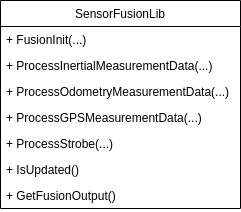
\includegraphics[width=0.7\linewidth]{img/SensorFusionLib}
	\caption{API di \textit{SensorFusionLib}}
	\label{fig:sfaapi}
\end{figure}
\section{Listener}
\textit{SensorFusionLib} \`e incapsulato all'interno di un eseguibile, \textit{listener}.\\*
Questo software possiede un'istanza di \textit{SensorFusionLib} con la quale interagisce attraverso le \texttt{API} descritte in 3.1.1. Esso dispone di due \textit{socket UDP}, una utilizzata per ricevere i dati \textit{raw} provenienti dai sensori, l'altra per la comunicazione remota con OBCU.
\begin{figure}[h]
	\centering
	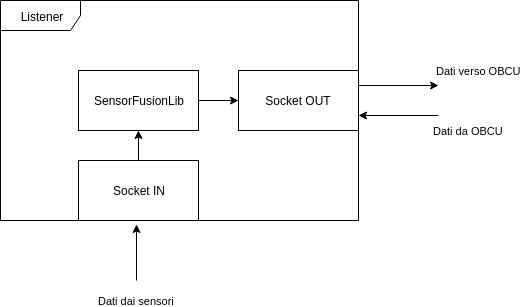
\includegraphics[width=0.7\linewidth]{img/ListenerOK}
	\caption{Architettura \emph{listener}}
	\label{fig:listener}
\end{figure}
\subsection{Database Interface}
Come anticipato nel capitolo 2, un ulteriore ingresso a SFA \`e rappresentato dalle informazioni geografiche della traccia su cui si trova il treno.\\*
Prima di poter inizializzare SFA attraverso una chiamata a \texttt{FusionInit()}, occorre specificare il database da utilizzare, e la classe concreta che implementa la comunicazione con esso.\\*
\emph{SensorFusionLib} contiene una classe astratta \texttt{DatabaseInterfaceEdges} implementata da due classi concrete:
\begin{itemize}
	\item \texttt{SQLITEDatabaseInterfaceEdges}, da utilizzare per connessioni verso un database \textit{sqlite};
	\item \texttt{MYSQLDatabaseInterfaceEdges}, da utilizzare per connessioni verso un database \textit{MySql}.
\end{itemize}
\begin{figure}[h]
	\centering
	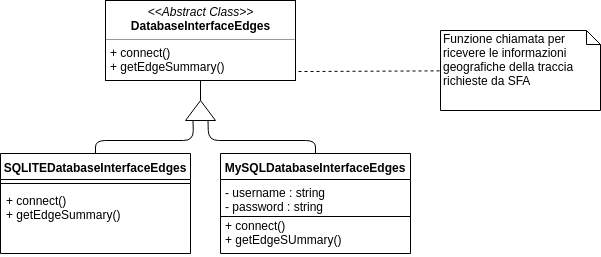
\includegraphics[width=0.7\linewidth]{img/dbintface}
	\caption{Class diagram \texttt{DatabaseInterfaceEdges}}
	\label{fig:dbiface}
\end{figure}
Quando \emph{SensorFusionLib} viene eseguito a bordo treno, deve essere specificato un file \textit{sqlite} che contiene il database da caricare in memoria centrale.\\*
Il software \emph{listener} ricerca automaticamente un file \textit{sqlite} nella \emph{directory} in cui si trova l'eseguibile, ed istanzia una connessione verso di esso utilizzando la classe concreta \texttt{SQLITEDatabaseInterfaceEdges}.\\*
SFA modella la determinata traccia ferrotramviaria lungo la quale si vuole eseguire l'algoritmo, come una \emph{spline} interpolante una lista di \emph{punti} sulla superficie della Terra.\\*
All'interno del database, ciascuna traccia \`e memorizzata in una tabella \emph{edges}.\\*
Una tabella \emph{edge\_vertices} memorizza le informazioni di progressiva chilometrica caratteristiche di ciascun punto geografico, associandolo alla traccia di appartenenza.\\*
Un'ultima tabella \emph{vertices} associa a ciascun punto geografico le sue coordinate \emph{ECEF}.
\begin{figure}[h]
	\centering
	\includegraphics[width=0.7\linewidth]{../Trainpositioning/train-positioning-tools/Documentation/SplineDatabaseSchema}
	\caption{Schema database tracce}
	\label{fig:dbschema}
\end{figure}\newpage
\section{Interface Modules}
La comunicazione con i sensori \`e gestita interamente da un set di processi denominati \textit{interface-modules}. Ciascun sensore \`e collegato ad un'interfaccia seriale della piattaforma attraverso un bus dati.
Per ogni interfaccia connessa, un processo resta in ascolto su di essa. Quando un sensore invia un campionamento su una specifica interfaccia, il processo in ascolto su quest'utlima si fa carico di inoltrare a \emph{listener} i valori ricevuti.\\*
Ciascun processo di \emph{interface-modules} dispone di una \emph{socket UDP} che abilita la comunicazione con \emph{listener}.
\begin{table}[h]
	\centering
	\begin{tabular}{|c|c|c|}
		\hline 
		\textbf{Modulo} & \textbf{Sensore}  & \textbf{Dati Inviati a \emph{listener}} \\ 
		\hline 
		\textit{IMU Process} & IMU & Accelerazione, Velocit\`a angolare \\ 
		\hline 
		\textit{ODO Process} & Odometro & Velocit\`a lineare  \\ 
		\hline 
		\textit{GPS Process} & GPS & Coordinate Geografiche \\ 
		\hline 
		\textit{Strobe Process} & N/A & Sincronizzazione \\ 
		\hline 
	\end{tabular}
	\caption{Moduli di \textit{interface-modules}}
	\label{tab:interfacem}
\end{table}
\begin{figure}[h]
	\centering
	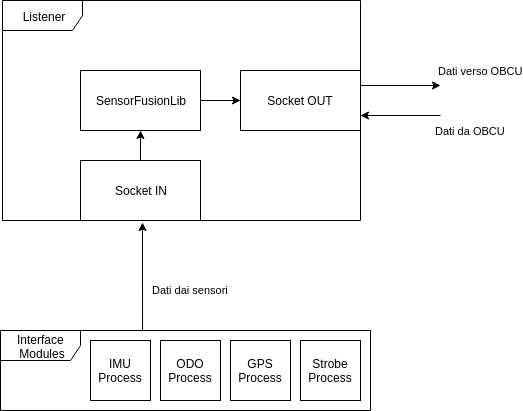
\includegraphics[width=0.7\linewidth]{img/IntModules}
	\caption{Architettura software completa}
	\label{fig:imod}
\end{figure}

